\section{NVIDIA系统管理接口（nvidia-smi）详解}

本章将解释 NVIDIA 系统管理接口（System Management Interface），即 \texttt{nvidia-smi}。
\texttt{nvidia-smi} 是 NVIDIA 提供的一个命令行工具，为 NVIDIA GPU 提供监控和管理功能，可实时检查 NVIDIA GPU 状态。本章将探讨 \texttt{nvidia-smi} 的一些关键特性及使用示例。

\subsection{nvidia-smi 的三大关键领域}

\texttt{nvidia-smi} 可用于三个关键领域：性能监控、设置管理和设备信息查询。

\begin{figure}
    \centering
    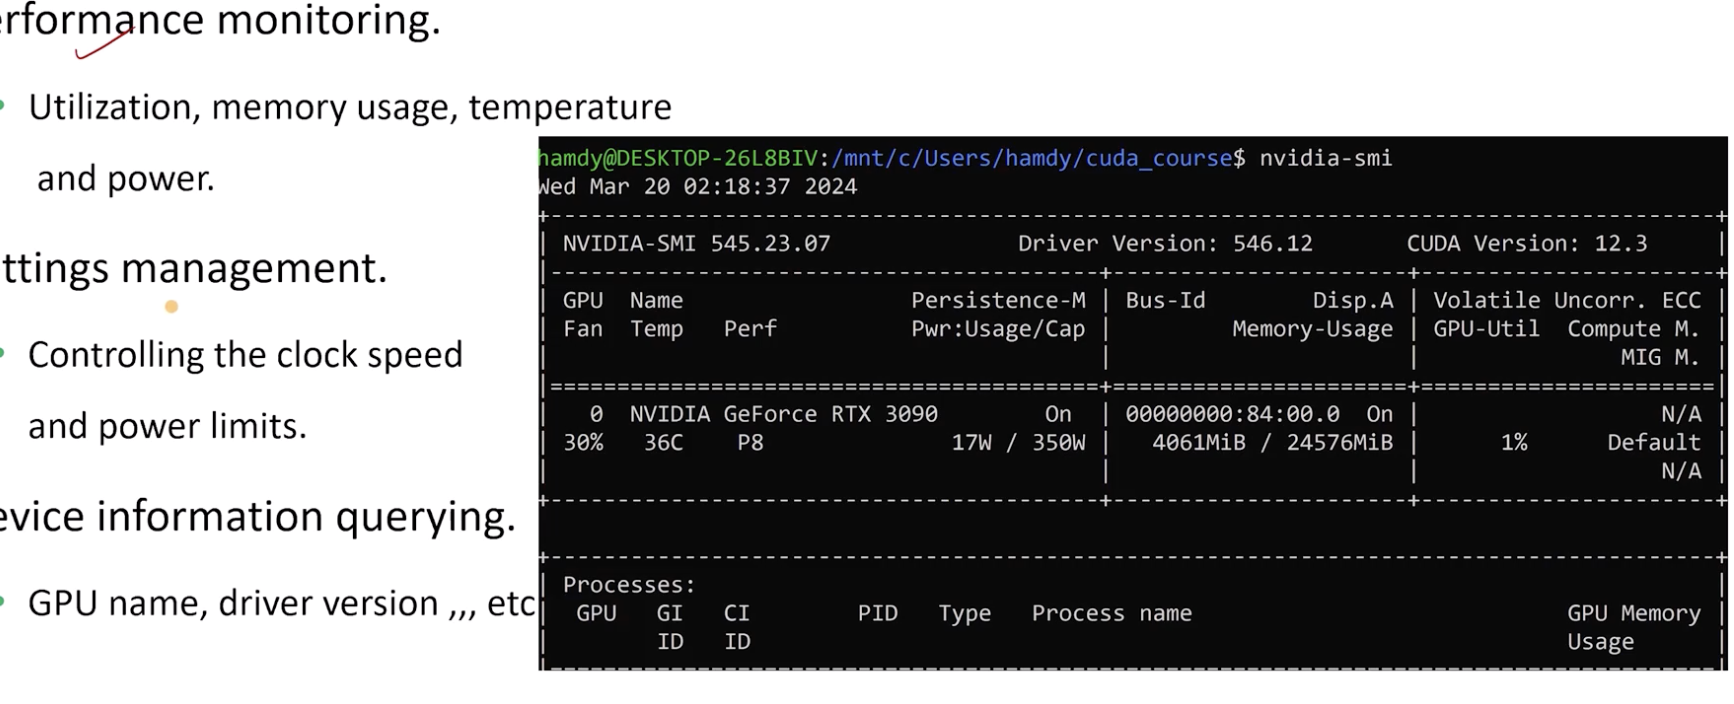
\includegraphics[width=0.75\linewidth]{resources/cuda-084.png}
    \caption{}
    \label{fig:placeholder}
\end{figure}

\begin{enumerate}
    \item \textbf{性能监控}: 可用于实时监控GPU性能，包括GPU资源利用率、内存使用情况、温度以及功耗。这些数据对于高效优化GPU资源至关重要。
    \item \textbf{设置管理}: 提供了调整或控制 GPU 内存和核心时钟速度的灵活性。不仅可以读取性能指标，还可以控制影响性能的参数。此外，可以为GPU功耗设定限制。
    \item \textbf{设备信息查询}: 提供关于GPU型号、驱动程序版本、CUDA版本以及当前时钟速度的全面详细信息。这确保开发者和管理员拥有必要的数据来做出关于软件兼容性和性能调优的明智决策。
\end{enumerate}

\subsection{基础命令与输出解读}

从最简单的命令开始：\texttt{nvidia-smi}。通过执行这个简单命令，我们可以获得性能指标的全面概览。
输出包含两个主要表格。

\subsection{第一个表格：性能概览}

第一行显示两个重要指标：
\begin{itemize}
    \item \textbf{驱动程序版本}: 例如 546.12。确认驱动版本有助于排查库兼容性问题。
    \item \textbf{CUDA版本}: 例如 12.3。可通过 \texttt{nvcc --version} 验证编译器版本是否匹配。
\end{itemize}

第二行是指标名称，第三行是对应值。该表格分为多列：
\begin{itemize}
    \item \textbf{GPU信息}: GPU名称（如 GeForce RTX 3090）、GPU ID（如 0）。
    \item \textbf{功耗与温度}: 当前功耗（如 31W）/ 最大功耗限制（如 350W）；当前温度（如 53°C）。
    \item \textbf{内存使用}: 已用显存 / 总显存（如 4000 MiB / 24 GiB）。
    \item \textbf{GPU 利用率}: 即使未运行自定义 CUDA 程序，若后台有录屏等应用调用 GPU 编码器，利用率也可能显示为 30\%-40\%。注意：\texttt{nvidia-smi} 的进程列表通常只显示 CUDA 计算进程，不一定显示视频编码/解码进程。
\end{itemize}

\begin{figure}
    \centering
    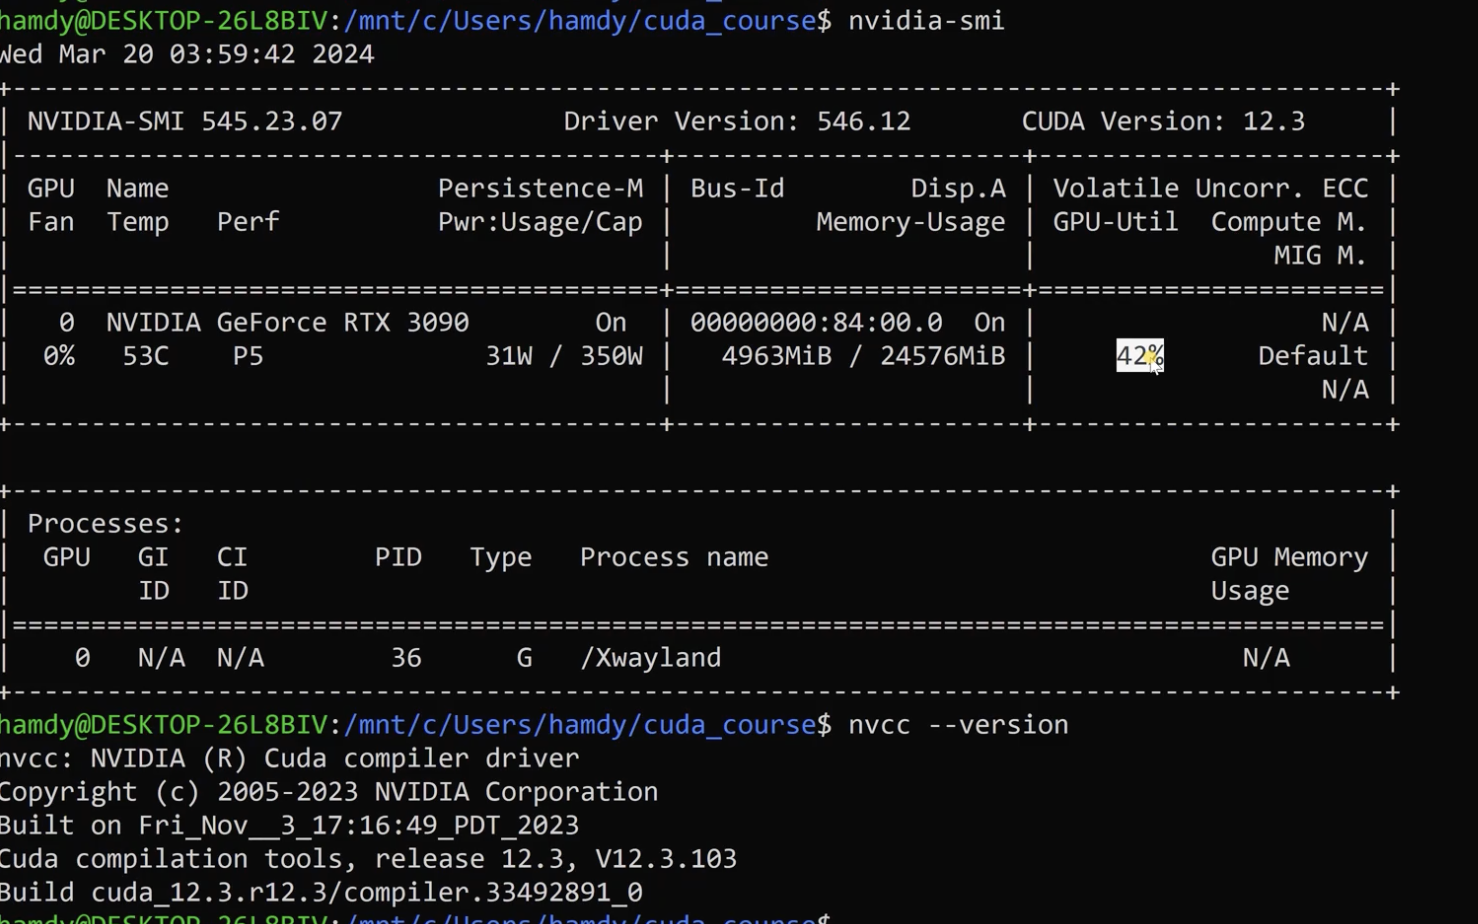
\includegraphics[width=0.75\linewidth]{resources/cuda-085.png}
    \caption{}
    \label{fig:placeholder}
\end{figure}

\subsection{第二个表格：进程列表}

此表格显示当前在GPU上运行的计算进程。例如运行矩阵乘法（Matrix Multiplication）应用时：
\begin{itemize}
    \item GPU利用率从空闲时的 $\sim$19\% 升至 100\%。
    \item 功耗从 $\sim$29W 升至 $\sim$318W（接近350W上限）。
    \item 温度从 36°C 升至 63°C。
    \item 显存占用显著增加（如增至 $\sim$8 GiB）。
\end{itemize}

\begin{figure}
    \centering
    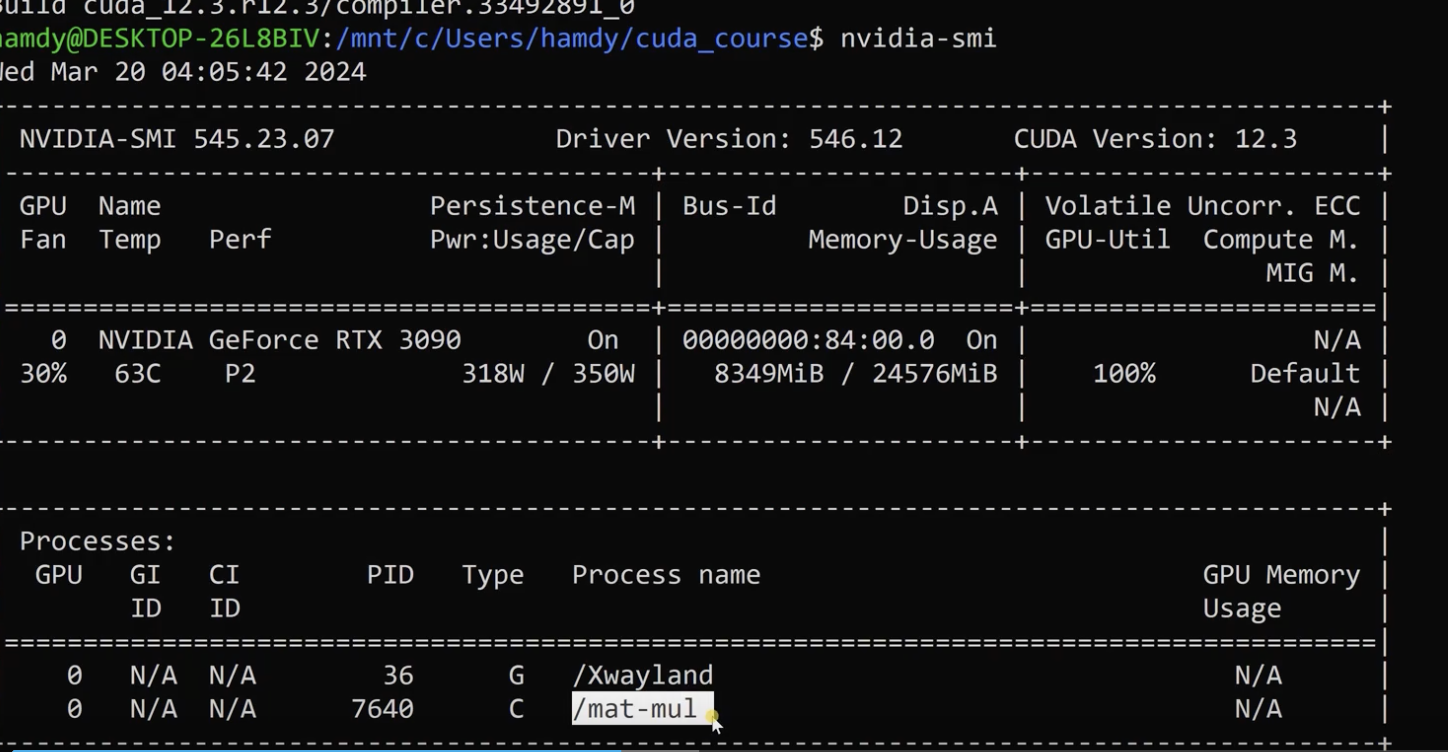
\includegraphics[width=0.75\linewidth]{resources/cuda-086.png}
    \caption{}
    \label{fig:placeholder}
\end{figure}

\subsection{持续监控与数据导出}

\subsection{循环查询模式}

使用 \texttt{-l} (loop) 参数实现持续监控：
\begin{lstlisting}
# 每5秒刷新一次
nvidia-smi -l 5

# 每2秒刷新一次
nvidia-smi -l 2
\end{lstlisting}
按 \texttt{Ctrl+C} 退出。通过对比刷新间隔内的数值变化，可以观察应用程序执行期间的实时性能波动。

\begin{figure}
    \centering
    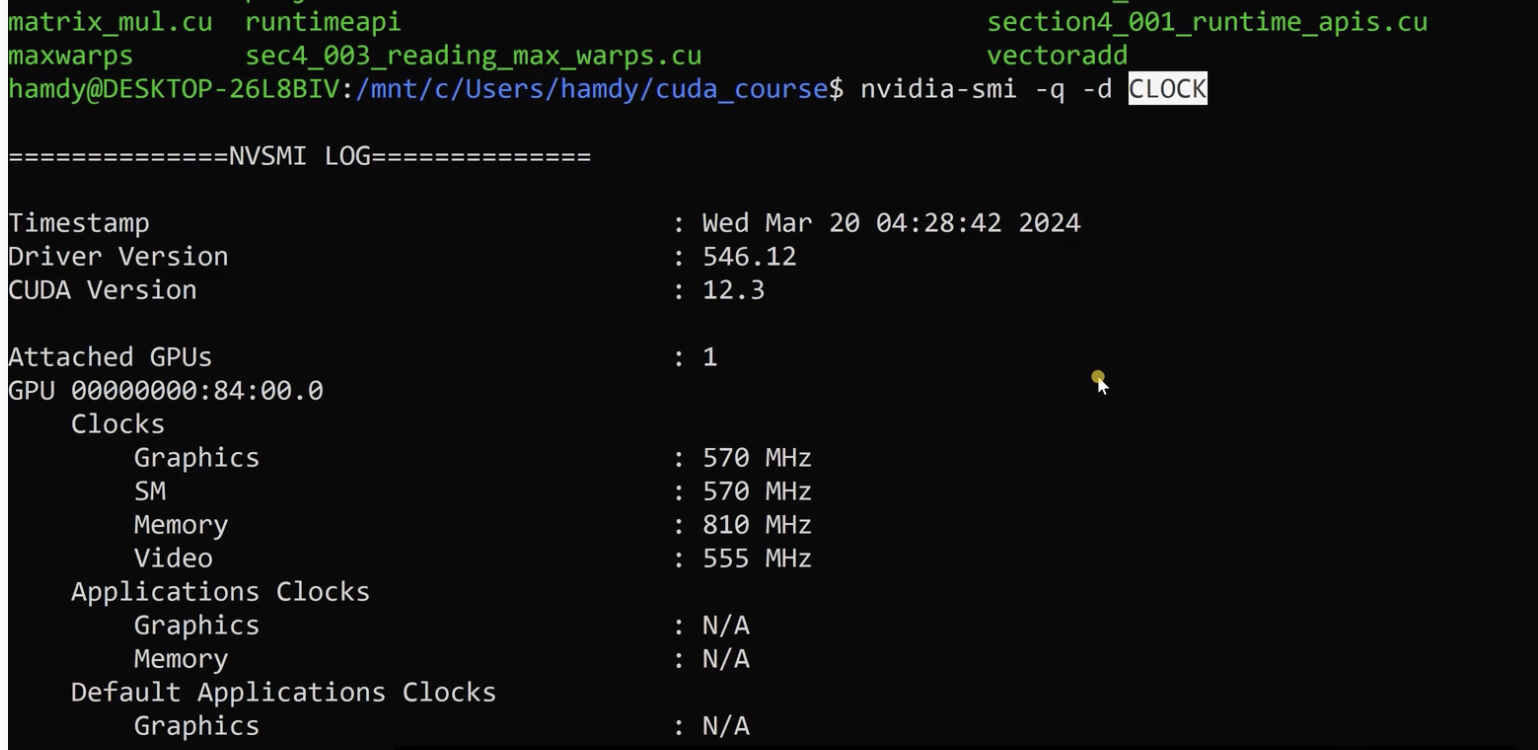
\includegraphics[width=0.75\linewidth]{resources/cuda-087.png}
    \caption{}
    \label{fig:placeholder}
\end{figure}

\subsection{定向查询与CSV导出}

使用 \texttt{--query-gpu} 和 \texttt{--format} 参数提取特定指标：
\begin{lstlisting}
# 查询指定指标并以CSV格式输出
nvidia-smi --query-gpu=name,driver_version,temperature.gpu \
           --format=csv

# 将结果保存到文件（Linux重定向）
nvidia-smi --query-gpu=name,driver_version,temperature.gpu \
           --format=csv > gpu_stats.csv
\end{lstlisting}
输出的CSV文件可直接用Excel打开进行分析。

\subsection{设置管理：功耗与时钟控制}

\subsection{功耗限制}

\begin{figure}
    \centering
    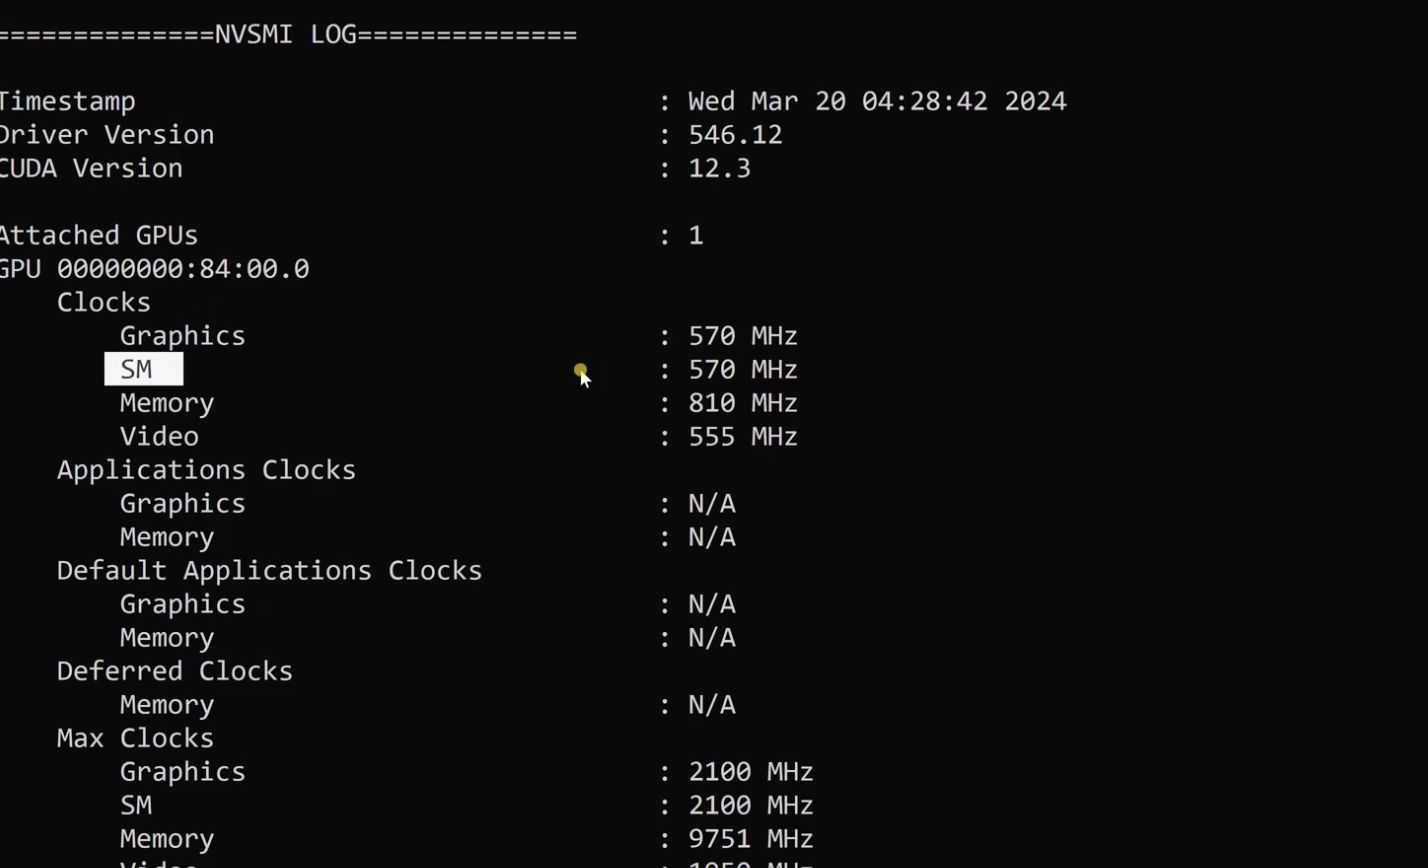
\includegraphics[width=0.75\linewidth]{resources/cuda-088.png}
    \caption{}
    \label{fig:placeholder}
\end{figure}

使用 \texttt{-pl} (power limit) 设置功耗上限：
\begin{lstlisting}
# 将GPU 0的功耗限制设为200W
sudo nvidia-smi -i 0 -pl 200
\end{lstlisting}
\textbf{注意}: 并非所有GPU都支持修改功耗限制，需提前确认硬件支持情况。

\subsection{持久模式（Persistence Mode）}

持久模式保持GPU驱动常驻内存，避免频繁加载/卸载开销。修改时钟等设置前可能需要先启用：
\begin{lstlisting}
# 启用持久模式
sudo nvidia-smi -i 0 -pm 1

# 禁用持久模式
sudo nvidia-smi -i 0 -pm 0
\end{lstlisting}

\subsection{时钟速度查询与控制}

\begin{figure}
    \centering
    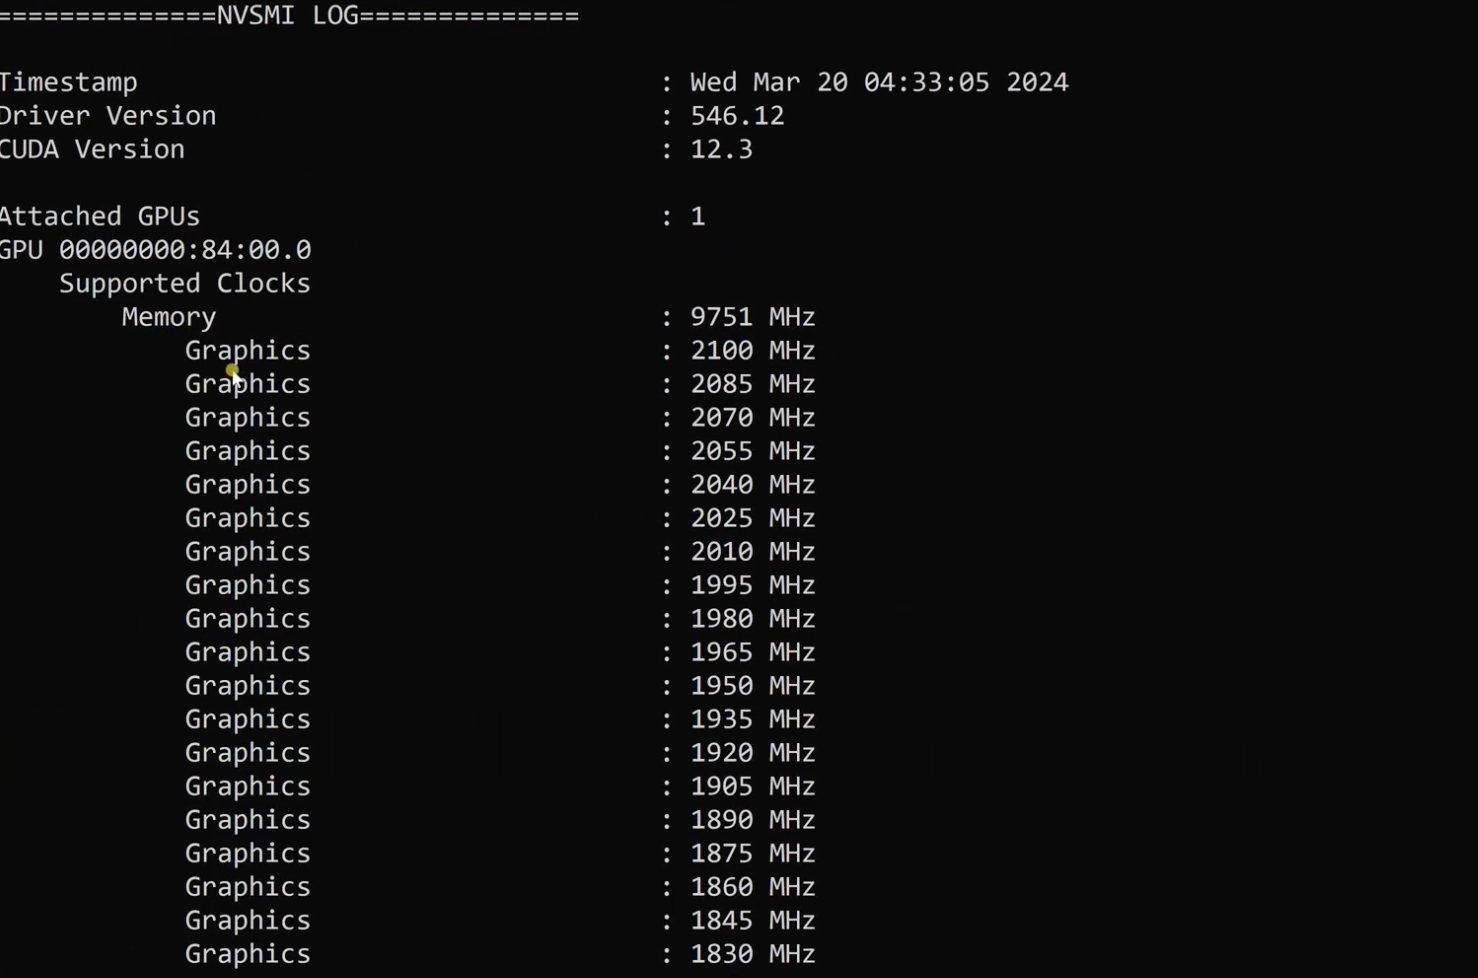
\includegraphics[width=0.75\linewidth]{resources/cuda-089.png}
    \caption{}
    \label{fig:placeholder}
\end{figure}


\subsection{查询时钟}

使用 \texttt{-q} (query) 查看时钟详情：
\begin{lstlisting}
nvidia-smi -q -d CLOCK
\end{lstlisting}
输出区分“当前时钟”与“最大时钟”。空闲时 GPU 会自动降频节能（如 SM 时钟从 2100 MHz 降至 570 MHz）；负载增加时自动升频（如升至 1695 MHz）。

\begin{lstlisting}
colin@colin-BATTLE-AX-B860M-P-WIFI:~$ nvidia-smi -q -d CLOCK

==============NVSMI LOG==============

Timestamp                                              : Sat Sep 26 11:19:58 2026
Driver Version                                         : 595.84
CUDA Version                                           : 13.2

Attached GPUs                                          : 1
GPU 00000000:02:00.0
    Clocks
        Graphics                                       : 180 MHz
        SM                                             : 180 MHz
        Memory                                         : 405 MHz
        Video                                          : 600 MHz
    Applications Clocks
        Graphics                                       : Requested functionality has been deprecated
        Memory                                         : Requested functionality has been deprecated
    Default Applications Clocks
        Graphics                                       : Requested functionality has been deprecated
        Memory                                         : Requested functionality has been deprecated
    Deferred Clocks
        Memory                                         : N/A
    Max Clocks
        Graphics                                       : 3090 MHz
        SM                                             : 3090 MHz
        Memory                                         : 14001 MHz
        Video                                          : 3090 MHz
    Max Customer Boost Clocks
        Graphics                                       : N/A
    SM Clock Samples
        Duration                                       : N/A
        Number of Samples                              : N/A
        Max                                            : N/A
        Min                                            : N/A
        Avg                                            : N/A
    Memory Clock Samples
        Duration                                       : N/A
        Number of Samples                              : N/A
        Max                                            : N/A
        Min                                            : N/A
        Avg                                            : N/A
    Clock Policy
        Auto Boost                                     : N/A
        Auto Boost Default                             : N/A
\end{lstlisting}

\subsection{查询支持的时钟频率}

设置固定时钟前，必须查询GPU支持的离散频率点：
\begin{lstlisting}
nvidia-smi -q -d SUPPORTED_CLOCKS
\end{lstlisting}
只能选择列表中存在的值（如内存 9501 MHz、5001 MHz；SM 12085 MHz、12070 MHz 等），不支持任意值。

\subsection{设置应用时钟}

使用 \texttt{-ac} (application clocks) 锁定SM和内存时钟：
\begin{lstlisting}
# 格式: -ac <mem_clock>,<sm_clock>
sudo nvidia-smi -i 0 -ac 9501,12085
\end{lstlisting}

\subsection{重置为默认值}

使用 \texttt{-r} 或 \texttt{-rac} / \texttt{-pmc} 重置设置：
\begin{lstlisting}
# 重置应用时钟为默认
sudo nvidia-smi -i 0 -rac

# 重置功耗限制为默认
sudo nvidia-smi -i 0 -pmc
\end{lstlisting}

\subsection{帮助与总结}

\begin{figure}
    \centering
    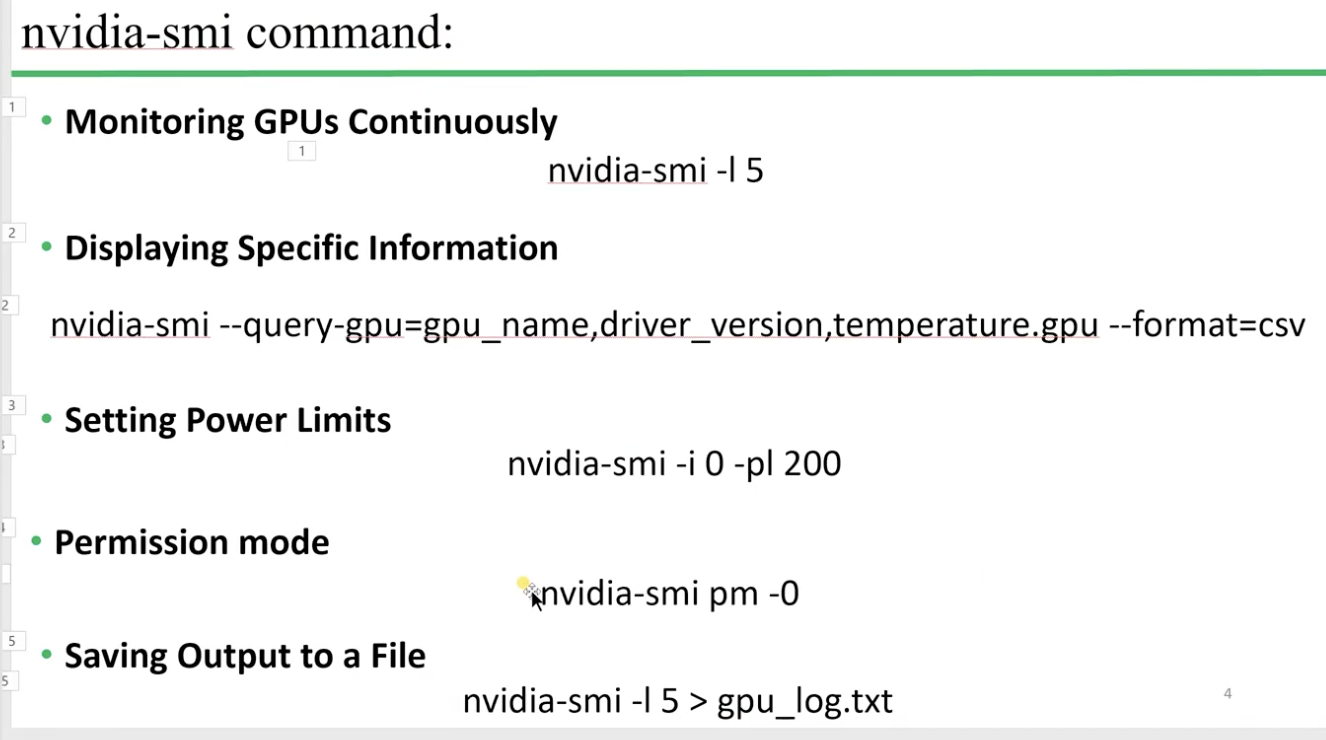
\includegraphics[width=0.75\linewidth]{resources/cuda-090.png}
    \caption{}
    \label{fig:placeholder}
\end{figure}

查看所有可用选项：
\begin{lstlisting}
nvidia-smi -h
\end{lstlisting}

\begin{lstlisting}
colin@colin-BATTLE-AX-B860M-P-WIFI:~$ nvidia-smi -h
NVIDIA System Management Interface -- v595.84

NVSMI provides monitoring information for Tesla and select Quadro devices.
The data is presented in either a plain text or an XML format, via stdout or a file.
NVSMI also provides several management operations for changing the device state.

Note that the functionality of NVSMI is exposed through the NVML C-based
library. See the NVIDIA developer website for more information about NVML.
Python wrappers to NVML are also available.  The output of NVSMI is
not guaranteed to be backwards compatible; NVML and the bindings are backwards
compatible.

http://developer.nvidia.com/nvidia-management-library-nvml/
http://pypi.python.org/pypi/nvidia-ml-py/
Supported products:
- Full Support
    - All Tesla products, starting with the Kepler architecture
    - All Quadro products, starting with the Kepler architecture
    - All GRID products, starting with the Kepler architecture
    - GeForce Titan products, starting with the Kepler architecture
- Limited Support
    - All Geforce products, starting with the Kepler architecture
nvidia-smi [OPTION1 [ARG1]] [OPTION2 [ARG2]] ...

    -h,   --help                Print usage information and exit.

          --version             Print version information and exit.

  LIST OPTIONS:

    -L,   --list-gpus           Display a list of GPUs connected to the system.

    -B,   --list-excluded-gpus  Display a list of excluded GPUs in the system.

  SUMMARY OPTIONS:

    <no arguments>              Show a summary of GPUs connected to the system.

    -col, --columns             Show a summary of GPUs connected to the system in multi-column format.

    [plus any of]

    -i,   --id=                 Target a specific GPU.
    -f,   --filename=           Log to a specified file, rather than to stdout.
    -l,   --loop=               Probe until Ctrl+C at specified second interval.

  QUERY OPTIONS:

    -q,   --query               Display GPU or Unit info.

    [plus any of]

    -u,   --unit                Show unit, rather than GPU, attributes.
    -i,   --id=                 Target a specific GPU or Unit.
    -f,   --filename=           Log to a specified file, rather than to stdout.
    -x,   --xml-format          Produce XML output.
          --dtd                 When showing xml output, embed DTD.
    -d,   --display=            Display only selected information: MEMORY,
                                    UTILIZATION, ECC, TEMPERATURE, POWER, CLOCK,
                                    COMPUTE, PIDS, PERFORMANCE, SUPPORTED_CLOCKS,
                                    PAGE_RETIREMENT, ACCOUNTING, ENCODER_STATS,
                                    SUPPORTED_GPU_TARGET_TEMP, VOLTAGE, FBC_STATS
                                    ROW_REMAPPER, GSP_FIRMWARE_VERSION
                                    POWER_SMOOTHING, POWER_PROFILES
                                Flags can be combined with comma e.g. ECC,POWER.
                                Sampling data with max/min/avg is also returned
                                for POWER, UTILIZATION and CLOCK display types.
                                Doesn't work with -u or -x flags.
    -l,   --loop=               Probe until Ctrl+C at specified second interval.

    -lms, --loop-ms=            Probe until Ctrl+C at specified millisecond interval.

  SELECTIVE QUERY OPTIONS:

    Allows the caller to pass an explicit list of properties to query.

    [one of]

    --query-gpu                 Information about GPU.
                                Call --help-query-gpu for more info.
    --query-supported-clocks    List of supported clocks.
                                Call --help-query-supported-clocks for more info.
    --query-compute-apps        List of currently active compute processes.
                                Call --help-query-compute-apps for more info.
    --query-accounted-apps      List of accounted compute processes.
                                Call --help-query-accounted-apps for more info.
                                This query is not supported on vGPU host.
    --query-retired-pages       List of device memory pages that have been retired.
                                Call --help-query-retired-pages for more info.
    --query-remapped-rows       Information about remapped rows.
                                Call --help-query-remapped-rows for more info.

    [mandatory]

    --format=                   Comma separated list of format options:
                                  csv - comma separated values (MANDATORY)
                                  noheader - skip the first line with column headers
                                  nounits - don't print units for numerical
                                             values

    [plus any of]

    -i,   --id=                 Target a specific GPU or Unit.
    -f,   --filename=           Log to a specified file, rather than to stdout.
    -l,   --loop=               Probe until Ctrl+C at specified second interval.
    -lms, --loop-ms=            Probe until Ctrl+C at specified millisecond interval.

  DEVICE MODIFICATION OPTIONS:

    [any one of]

    -pm,  --persistence-mode=   Set persistence mode: 0/DISABLED, 1/ENABLED
    -e,   --ecc-config=         Toggle ECC support: 0/DISABLED, 1/ENABLED
    -p,   --reset-ecc-errors=   Reset ECC error counts: 0/VOLATILE, 1/AGGREGATE
    -c,   --compute-mode=       Set MODE for compute applications:
                                0/DEFAULT, 1/EXCLUSIVE_THREAD (DEPRECATED),
                                2/PROHIBITED, 3/EXCLUSIVE_PROCESS
          --gom=                Set GPU Operation Mode:
                                    0/ALL_ON, 1/COMPUTE, 2/LOW_DP
    -r    --gpu-reset           Trigger reset of the GPU.
                                Can be used to reset the GPU HW state in situations
                                that would otherwise require a machine reboot.
                                Typically useful if a double bit ECC error has
                                occurred.
                                Reset operations are not guaranteed to work in
                                all cases and should be used with caution.
                                Reset triggered without extra arguments, will be a.
                                default Function Level Reset (FLR). To issue a
                                Bus Reset, use -r bus.
    -vm   --virt-mode=          Switch GPU Virtualization Mode:
                                Sets GPU virtualization mode to 3/VGPU or 4/VSGA
                                Virtualization mode of a GPU can only be set when
                                it is running on a hypervisor.
    -lgc  --lock-gpu-clocks=    Specifies <minGpuClock,maxGpuClock> clocks as a
                                    pair (e.g. 1500,1500) that defines the range
                                    of desired locked GPU clock speed in MHz.
                                    Setting this will supersede application clocks
                                    and take effect regardless if an app is running.
                                    Input can also be a singular desired clock value
                                    (e.g. <GpuClockValue>). Optionally, --mode can be
                                    specified to indicate a special mode.
    -m    --mode=               Specifies the mode for --lock-gpu-clocks.
                                    Valid modes: 0, 1
    -rgc  --reset-gpu-clocks
                                Resets the GPU clocks to the default values.
    -lmc  --lock-memory-clocks=  Specifies <minMemClock,maxMemClock> clocks as a
                                    pair (e.g. 5100,5100) that defines the range
                                    of desired locked Memory clock speed in MHz.
                                    Input can also be a singular desired clock value
                                    (e.g. <MemClockValue>).
    -rmc  --reset-memory-clocks
                                Resets the Memory clocks to the default values.
    -lmcd --lock-memory-clocks-deferred=
                                    Specifies memClock clock to lock. This limit is
                                    applied the next time GPU is initialized.
                                    This is guaranteed by unloading and reloading the kernel module.
                                    Requires root.
    -rmcd --reset-memory-clocks-deferred
                                Resets the deferred Memory clocks applied.
    -ac   --applications-clocks= Specifies <memory,graphics> clocks as a
                                    pair (e.g. 2000,800) that defines GPU's
                                    speed in MHz while running applications on a GPU.
    -rac  --reset-applications-clocks
                                Resets the applications clocks to the default values.
    -pl   --power-limit=        Specifies maximum power management limit in watts.
                                Takes an optional argument --scope.
    -sc   --scope=              Specifies the device type for --scope: 0/GPU, 1/TOTAL_MODULE (Grace Hopper Only)
    -cc   --cuda-clocks=        Overrides or restores default CUDA clocks.
                                In override mode, GPU clocks higher frequencies when running CUDA applications.
                                Only on supported devices starting from the Volta series.
                                Requires administrator privileges.
                                0/RESTORE_DEFAULT, 1/OVERRIDE
    -am   --accounting-mode=    Enable or disable Accounting Mode: 0/DISABLED, 1/ENABLED
    -caa  --clear-accounted-apps
                                Clears all the accounted PIDs in the buffer.
          --auto-boost-default= Set the default auto boost policy to 0/DISABLED
                                or 1/ENABLED, enforcing the change only after the
                                last boost client has exited.
          --auto-boost-permission=
                                Allow non-admin/root control over auto boost mode:
                                0/UNRESTRICTED, 1/RESTRICTED
    -mig  --multi-instance-gpu= Enable or disable Multi Instance GPU: 0/DISABLED, 1/ENABLED
                                Requires root.
    -gtt  --gpu-target-temp=    Set GPU Target Temperature for a GPU in degree celsius.
                                Requires administrator privileges
    -den, --dram-encryption=    Toggle DRAM Encryption support: 0/DISABLED, 1/ENABLED
                                Requires root.
           --set-hostname=      Set the hostname associated with the GPU.
                                Requires root.
           --get-hostname       Get the hostname associated with the GPU.

   [plus optional]

    -i,   --id=                 Target a specific GPU.
    -eow, --error-on-warning    Return a non-zero error for warnings.

  UNIT MODIFICATION OPTIONS:

    -t,   --toggle-led=         Set Unit LED state: 0/GREEN, 1/AMBER

   [plus optional]

    -i,   --id=                 Target a specific Unit.

  SHOW DTD OPTIONS:

          --dtd                 Print device DTD and exit.

     [plus optional]

    -f,   --filename=           Log to a specified file, rather than to stdout.
    -u,   --unit                Show unit, rather than device, DTD.

    --debug=                    Log encrypted debug information to a specified file.

 Device Monitoring:
    dmon                        Displays device stats in scrolling format.
                                "nvidia-smi dmon -h" for more information.

    daemon                      Runs in background and monitor devices as a daemon process.
                                This is an experimental feature. Not supported on Windows baremetal
                                "nvidia-smi daemon -h" for more information.

    replay                      Used to replay/extract the persistent stats generated by daemon.
                                This is an experimental feature.
                                "nvidia-smi replay -h" for more information.

 Process Monitoring:
    pmon                        Displays process stats in scrolling format.
                                "nvidia-smi pmon -h" for more information.

 TOPOLOGY:
    topo                        Displays device/system topology. "nvidia-smi topo -h" for more information.

 DRAIN STATES:
    drain                       Displays/modifies GPU drain states for power idling. "nvidia-smi drain -h" for more information.

 NVLINK:
    nvlink                      Displays device nvlink information. "nvidia-smi nvlink -h" for more information.

 C2C:
    c2c                         Displays device C2C information. "nvidia-smi c2c -h" for more information.

 CLOCKS:
    clocks                      Control and query clock information. "nvidia-smi clocks -h" for more information.

 ENCODER SESSIONS:
    encodersessions             Displays device encoder sessions information. "nvidia-smi encodersessions -h" for more information.

 FBC SESSIONS:
    fbcsessions                 Displays device FBC sessions information. "nvidia-smi fbcsessions -h" for more information.

 GRID vGPU:
    vgpu                        Displays vGPU information. "nvidia-smi vgpu -h" for more information.

 MIG:
    mig                         Provides controls for MIG management. "nvidia-smi mig -h" for more information.

 COMPUTE POLICY:
    compute-policy              Control and query compute policies. "nvidia-smi compute-policy -h" for more information.

 BOOST SLIDER:
    boost-slider                Control and query boost sliders. "nvidia-smi boost-slider -h" for more information.

 POWER HINT:
    power-hint                  Estimates GPU power usage. "nvidia-smi power-hint -h" for more information.

 BASE CLOCKS:
    base-clocks                 Query GPU base clocks. "nvidia-smi base-clocks -h" for more information.

 CONFIDENTIAL COMPUTE:
    conf-compute                Control and query confidential compute. "nvidia-smi conf-compute -h" for more information.

 GPU PERFORMANCE MONITORING:
    gpm                         Control and query GPU performance monitoring unit. "nvidia-smi gpm -h" for more information.

 PCI:
    pci                         Display device PCI information. "nvidia-smi pci -h" for more information.

 Power Smoothing:
    power-smoothing             Control and query power smoothing information. "nvidia-smi power-smoothing -h" for more information.

 Power Profiles:
    power-profiles              Control and query workload power profiles information. "nvidia-smi power-profiles -h" for more information.

 RUSD:
    rusd                         Set RUSD (read only shared data buffer) settings. "nvidia-smi rusd -h" for more information.

 PRM:
    prm                         Query GPU PRM registers. "nvidia-smi prm -h" for more information.

 SOC:
    soc                          Query system on chip metrics. "nvidia-smi soc -h" for more information.

Please see the nvidia-smi(1) manual page for more detailed information.
\end{lstlisting}

\texttt{nvidia-smi} 是一个非常重要的命令。在后续章节中，将使用 \texttt{nvidia-smi} 来检查各种性能指标，验证优化效果，并诊断 GPU 运行状态。
